\chapter{Технологические карты}

\newcounter{techcard}

\newcommand{\techcardsection}[1]{
    \refstepcounter{techcard}
    \label{techcard\arabic{techcard}}
    \section{#1}
}

\techcardsection{Промывка топливного фильтра грубой (предварительной) очистки}
Исполнитель: механик-водитель. 

Инструмент и приспособления: ключи гаечные 12, 17, 19, 22 и 24~мм; плоскогубцы, отвертка, кружка для слива топлива, ванна, кисть волосяная. 

Норма времени~--- 17 мин.

\subsubsection{Содержание работ и технические условия}
\begin{enumerate}
    \item Поставить топливораспределительный кран в положение выключения топливных баков. 
    \item Открыть надмоторный люк и зафиксировать его крышку в открытом положении стопором. 
    \item Открыть пробки 9 (рис.~\ref{filter}) заливного и 1 сливного отверстий и слить топливо из корпуса 3 фильтра. Завернуть пробку 1 сливного отверстия. 
    \item Отвернуть четыре болта 8 крепления корпуса 3 к крышке 6, снять корпус и вынуть из него фильтрующий элемент 4. 
    \item Промыть дизельным топливом внутренние поверхности корпуса 3, крышки 6 и фильтрующий элемент 4. 
    \item Вставить в корпус 3 фильтрующий элемент 4, присоединить корпус к крышке 6 и закрепить болтами 8. 
    \item Залить в фильтр чистое топливо и завернуть пробку 9 заливного отверстия. 
    \item Топливораспределительный кран поставить в положение включения топливных баков. 
    \item Пустить двигатель и проверить его работу. При перебоях в работе, подсасывании воздуха подтянуть болты крепления фильтра, прокачать систему насосом РНМ-1А. 
    \item Закрыть надмоторный люк, освободив крышку от стопора
\end{enumerate}

\begin{figure}[h]
    \begin{center}
        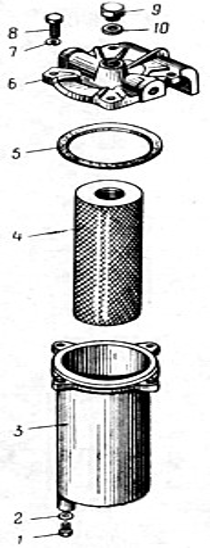
\includegraphics[width=0.3\textwidth]{src/filter.png}
        \caption{Фильтр грубой очистки топлива}
        \label{filter}
    \end{center}
    \legend
    1 и 9~--- пробки; 2 и 7~--- шайбы; 3~--- корпус фильтра; 4~--- фильтрующий элемент; 5~--- прокладка крышки; 6~--- крышка; 8~--- болт; 10~--- прокладка
\end{figure}



\techcardsection{Промывка топливного фильтра тонкой очистки}
Исполнитель: механик-водитель. 

Инструмент и приспособления: ключи гаечные 17, 19 и 24~мм; отвертки, кружка для слива топлива, ванна для промывки деталей, кисть волосяная, воронка малая. 

Норма времени~--- 15 мин.

\subsubsection{Содержание работ и технические условия}
\begin{enumerate}
\item Открыть надмоторный люк и зафиксировать его крышку в открытом положении стопором, открыть заднюю панель ограждения двигателя.
\item Отвернуть сливную 18 (рис.~\ref{soft_filter}) и коническую 3 пробки и слить топливо из корпуса 16 фильтра, после чего пробку 18 завернуть. 
\item Отвернуть болт 6 крепления корпуса 16 фильтра к крышке 2, снять корпус, вынуть из него старый фильтрующий элемент 12 и пружину 15. 
\item Промыть бензином или дизельным топливом внутренние поверхности корпуса фильтра, крышки и фильтрующий элемент. Если фильтрующий элемент стал мягким, заменить его новым. 
\item Поставить в корпус 16 пружину 15, шайбу 14, резиновую прокладку 13 и фильтрующий элемент 12 (металлическим фланцем вниз), на верхний фланец элемента установить резиновую прокладку 1. 
\item Поставить шайбу 7 болта 6 крепления и прокладку корпуса, установить корпус с фильтрующим элементом на место и тщательно затянуть болт 6. 
\item Залить в фильтр чистое топливо и завернуть коническую пробку 3 заливного отверстия. 
\item Пустить двигатель и проверить, не подтекает ли топливо в соединениях фильтра.При необходимости подтянуть болт 6 крепления корпуса. 
\item Закрыть надмоторный люк, освободив крышку от стопора, и панели ограждения двигателя

\end{enumerate}

\begin{figure}[h]
    \begin{center}
        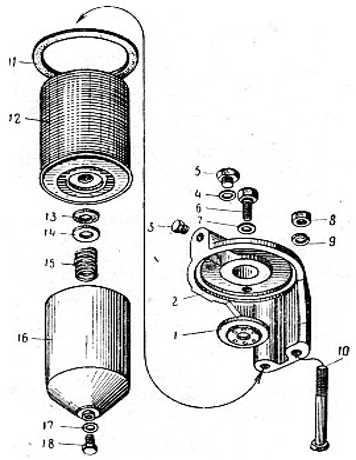
\includegraphics[width=0.65\textwidth]{src/soft_filter.png}
        \caption{Фильтр тонкой очистки топлива}
        \label{soft_filter}
    \end{center}
    \legend
    1, 4, 11, 13 и 17~--- прокладки; 2~--- крышка фильтра; 3 и 8~--- пробки; 5~--- жиклер; 6 и 10~--- болты; 7, 9 и 14~--- шайбы; 8~--- гайка; 12~--- фильтрующий элемент; 15~--- пружина; 16~--- корпус фильтра 
\end{figure}



\techcardsection{Промывка топливных баков}
\subsection{Промывка топливных баков без снятия с транспортера-тягача}
Исполнитель: механик-водитель.

Инструмент и приспособления: ключи гаечные 12 и 32~мм, ключ 12$\times$12~мм к пробкам картера бортовых передач и к сливным пробкам топливных баков; малогабаритный заправочный агрегат МЗА-3, шланг для слива топлива из топливных баков.

Норма времени~--- 90 мин. 

\subsubsection{Содержание работ и технические условия}
\begin{enumerate}
\item Отвернуть пробки заливных горловин топливных баков, предварительно протерев их от грязи, и вынуть сетчатые фильтры из заливных горловин. 
\item Отвернуть болты крепления крышек люков к. днищу корпуса и снять крышки люков под каждой группой топливных баков (рис.~\ref{bottom}). 
\item Ввернуть штуцер 6 (рис.~\ref{key}) со шлангом в корпус 7 сливной пробки 4, отвернуть ее на два-три оборота и слить топливо в подставленную тару. 
\item Промыть каждую группу баков с помощью малогабаритного заправочного агрегата МЗА-3 (рис.~\ref{zapravochniy}). Для этого вставить раздаточный кран 4 в заливную горловину промываемой группы баков, и в течение 0,5 мин нагнетать топливо в группу баков при максимальной производительности насоса (60~л/мин). 
\item Затянуть сливные пробки топливных баков после полного слива топлива из них. Установить крышки люков под топливными баками и прикрепить их болтами к днищу корпуса транспортера-тягача. 
\item Заправить топливные баки соответствующим сортом топлива.
\item Установить сетчатые фильтры в заливные горловины и ввернуть пробки в заливные горловины.
\end{enumerate}

\begin{figure}
    \begin{center}
        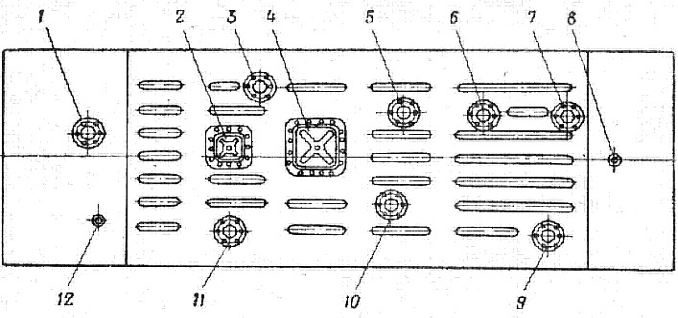
\includegraphics[width=\textwidth]{src/bottom.png}
        \caption{Днище рамы с люками (с наружной стороны)}
        \label{bottom}
    \end{center}
    \legend
    1~--- люк для слива масла из главной передачи; 2~--- люк для слива масла из картера промежуточного редуктора; 3~--- люк для слива масла из масляного бака главной передачи; 4~--- люк для слива масла из картера двигателя; 5, 6, 7 и 9~--- люки для слива топлива из топливных баков; 8 и 12~--- кингстоны; 10~--- люк для слива масла из картера лебедки;  11~--- люк для слива масла из реверс-редуктора 
\end{figure}

\begin{figure}
    \begin{center}
        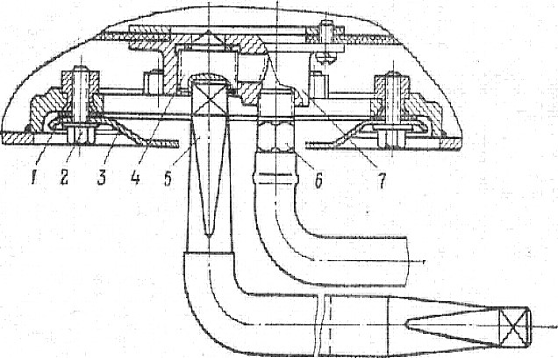
\includegraphics[width=0.65\textwidth]{src/key.png}
        \caption{Установка ключа и шланга для слива топлива из топливных баков}
        \label{key}
    \end{center}
    \legend
    1~--- прокладка; 2~--- болт; 3~--- крышка лючка; 4~--- сливная пробка; 5~--- ключ; 6~--- штуцер шланга; 7~--- корпус сливной пробки
\end{figure}

\begin{figure}
    \begin{center}
        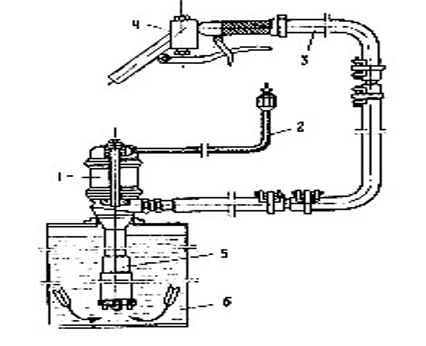
\includegraphics[width=0.65\textwidth]{src/zapravochniy.png}
        \caption{Малогабаритный заправочный агрегат МЗА-3}
        \label{zapravochniy}
    \end{center}
    \legend
    1~--- насос с электродвигателем; 2~--- электрокабель; 3~--- раздаточный шланг; 4 и 6~--- раздаточный емкость с топливом кран; 5~--- илиудлинитель маслом
\end{figure}


\subsection{Снятие топливных баков с транспортера-тягача, промывка и установка их}
Исполнители: механик-водитель и слесарь. 

Инструмент и приспособления: ключи гаечные 10, 12, 14, 17, 19, 27 и 32~мм, ключ 12$\times$12~мм к пробкам картера бортовых передач и сливным пробкам топливных баков; отвертка, плоскогубцы, шланг для слива топлива из топливных баков. 

Норма времени~--- для механика-водителя 240~мин, для слесаря 60~мин. 

\subsubsection{Содержание работ и технические условия}
\begin{enumerate}
    \item Отвернуть болты крепления крышек люков к днищу корпуса. 
    \item Снять крышки люков под каждой группой топливных баков (рис.~\ref{bottom}). 
    \item Ввернуть штуцер 6 (рис.~\ref{key}) со шлангом в корпус 7 сливной пробки 4, отвернуть ее на \range{два}{три} оборота и слить топливо в подставленную тару. 
    \item Снять сиденья и спинки сидений с нижних топливных баков. 
    \item Отвернуть пробку и винты крепления заливной горловины. 
    \item Отсоединить стяжные ленты, крепящие верхний топливный бак. 
    \item Отсоединить трубки подвода топлива и соединительные трубки между баками. 
    \item Снять верхний бак, сохранив прокладки постелей и хомутов бака. 
    \item Отсоединить трубки подвода и отвода топлива от нижнего топливного бака. 
    \item Отсоединить три верхних и два нижних прижима нижнего бака (расшплинтовать и отвернуть болты крепления прижимов топливного бака). 
    \item Снять нижний топливный бак. 
    \item Залить в каждый топливный бак по \range{15}{20}~л топлива и промыть топливные баки путем взбалтывания. 
    \item Установить топливные баки в обратной последовательности.
\end{enumerate}

\techcardsection{Промывка фильтра грубой очистки масла}
Исполнитель: механик-водитель.

Инструмент и приспособления: ключи гаечные 19, 24 и 27~мм; отвертка. 

Норма времени~--- 215~мин. 

\subsubsection{Содержание работ и технические условия}
\begin{enumerate}
    \item Снять боковую панель ограждени двигателя. 
    \item Вывернуть сливную пробку и слить масло из фильтра в подставленную тару, после чего пробку завернуть. 
    \item Отвернуть гайку 5 (рис.~\ref{filter_1}) колпака 4 фильтра и снять колпак, наружную 3 и внутреннюю 2 секции фильтрующих элементов. 

    \begin{figure}
        \begin{center}
            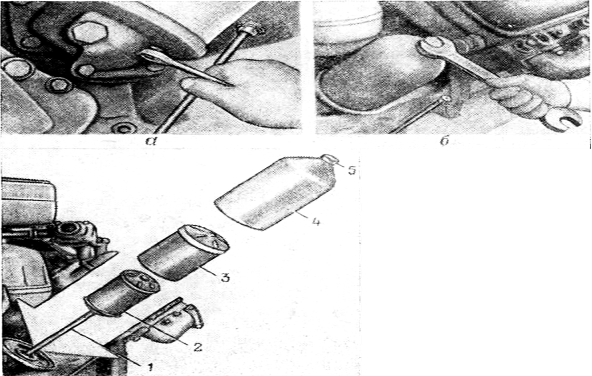
\includegraphics[width=0.8\textwidth]{src/filter_1.png}
            \caption{Фильтр грубой очистки масла}
            \label{filter_1}
        \end{center}
        \legend
        \begin{itemize}
            \item[a] вывертывание сливной пробки фильтра грубой очистки масла;
            \item[b] отвертывание гайки 5 колпака фильтра;
        \end{itemize}  
        1~--- стержень фильтра; 2 и 3~--- внутренняя и наружная секции фильтра; 4~--- колпак фильтра; 5~--- гайка крепления колпака 
    \end{figure}

    \item Поместить на 3 часа (не менее) секции в ванну с растворителем (бензином или четыреххлористым углеродом). 

    \textbf{Внимание!} Четыреххлористый углерод ядовит, поэтому при обращении с ним необходимо соблюдать осторожность. 
    \item Промыть элементы мягкой волосяной щеткой в ванне с растворителем. 
    \item Поместить элементы в ванну с чистым бензином или четыреххлористым углеродом, прополоскать каждый элемент и затем продуть сжатым воздухом. 

    Фильтрующие элементы можно также прокипятить в 10\% водном растворе каустической соды, затем промыть в дизельном топливе и продуть сжатым воздухом. Время кипячения~--- от 30~мин до 6 часов зависимости от степени их загрязнения. 
    \item Промыть в дизельном топливе колпак 4 фильтра. 
    \item Собрать фильтр, для чего надеть на стержень 1 секции 2 и 3 фильтрующих элементов, затем колпак 4 и тщательно затянуть гайку 5. 
    \item Поставить на место боковую панель ограждения двигателя. 

\end{enumerate}

\techcardsection{Промывка фильтра центробежной (тонкой) очистки масла}
Исполнитель: механик-водитель. 

Инструмент и приспособления: ключи гаечные 17, 19 и 24~мм; отвертка. 

Норма времени~--- 25~мин. 

\begin{enumerate}
    \item Открыть надмоторный люк и зафиксировать его крышку в открытом положении стопором. 
    \item Отвернуть гайку 13 (рис.~\ref{filter_2}) колпака фильтра и снять колпак 11.
    
    \begin{figure}
        \begin{center}
            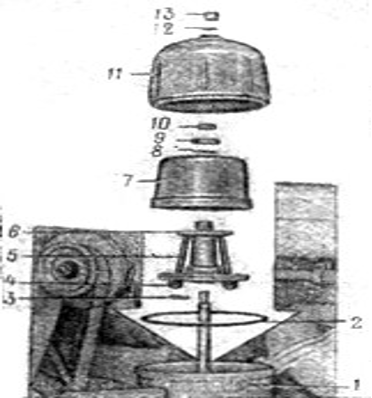
\includegraphics[width=0.6\textwidth]{src/filter_2.png}
            \caption{Фильтр центробежной (тонкой) очистки масла}
            \label{filter_2}
        \end{center}
        \legend
        1~--- корпус фильтра; 2~--- прокладка; 3~--- чека; 4~--- сопло ротора; 5~--- ротор; 6~--- сетка ротора; 7~--- колпак ротора; 8 и 12~--- шайбы; 9~и 13~--- гайки; 10~--- упорная шайба; 11~--- колпак фильтра  
    \end{figure}

    \item Снять упорную шайбу 10 и ротор в сборе и разобрать его, сняв гайку 9, шайбу 8, колпак 7 ротора. 
    \item Удалить с колпака 7 и ротора 5 осадок, промыв их в дизельном топливе. 
    \item Собрать фильтр в обратной последовательности, проверив состояние прокладки 2, сопел 4, ротора 5, упорной шайбы 10 и положение сетки 6. 
    
    При необходимости прокладку 2 заменить, сетку 6 поставить в нормальное положение, а сопла 4 ротора прочистить. 
    \item Закрыть надмоторный люк, освободив крышку от стопора. 

\end{enumerate}


\techcardsection{Замена масла и промывка системы смазки двигателя}
Исполнитель: механик-водитель. 

Инструмент и приспособления: ключи гаечные 12, 19, 24 и 36~мм; отвертка. 

Норма времени~--- 20 мин. 

\subsubsection{Содержание работ и технические условия}

\begin{enumerate}
    \item Пустить двигатель и прогреть его до температуры охлаждающей жидкости \celc{70}. 
    \item Снять боковую панель ограждения, двигателя, открыть надмоторный люк и зафиксировать его крышку в открытом положении стопором. 
    \item Отвернуть болты крепления и снять крышку подмоторного люка. 
    \item Снять крышку головки заливной горловины, отвернуть сливную пробку в поддоне двигателя, слить из поддона отработанное масло и завернуть сливную пробку. 
    \item Выполнить операции, предусмотренные Технологическими картами №\ref{techcard4} и \ref{techcard5}. 
    \item \begin{enumerate}
        \item Залить в систему смазки двигателя смесь из 10~л дизельного топлива и 6~л дизельного масла, запустить двигатель и поработать \range{4}{5}~мин на минимальных оборотах холостого хода, после чего слить промывочную смесь. 
        \item Повторно промыть фильтры (см. технологические карты №\ref{techcard4} и \ref{techcard5}). 
    \end{enumerate}
    \item Залить в систему свежее масло до отметки «В» на масломерном щупе, закрыть крышкой головку заливной горловины. 
    \item Поставить крышку подмоторного люка на место и закрепить ее болтами. 
    \item Закрыть надмоторный люк, освободив крышку от стопора, поставить на место боковую панель ограждения двигателя. 
\end{enumerate}

\techcardsection{Очистка и промывка воздухоочистителя}
Исполнитель: механик-водитель. 

Инструмент и приспособления: ключи гаечные 10, 17, 19 и 24~мм; отвертка, противень, скребок, шетка. 

Норма времени~--- 30~мин (с промывкой циклонов и бункера воздухоочистителя 50~мин). 

\subsubsection{Содержание работ и технические условия}

\begin{figure}
    \begin{center}
        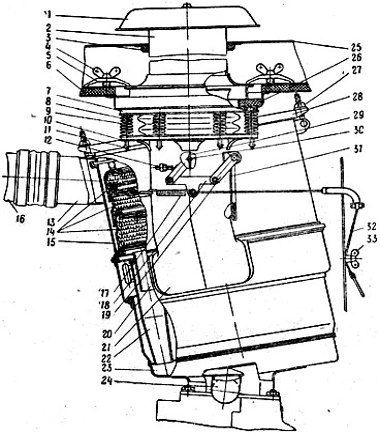
\includegraphics[width=0.7\textwidth]{src/air_filter.png}
        \caption{Воздухоочиститель}
        \label{air_filter}
    \end{center}
    \legend
    1~--- защитный колпак; 2 и 21~--- воздухозаборные патрубки; 3 и 26~--- уплотнения; 4 и 27~--- барашки; 5~--- прижим; 6~--- верхняя передняя панель ограждения двигателя; 7~--- уплотнитель; 8~--- пружина; 9~--- палец; 10~--- фланец; 11~--- шплинт; 12~--- винт упора; 13~--- патрубок отвода чистого воздуха; 14~--- кассета фильтрующего элемента; 15~--- корпус воздухоочистителя; 16~--- патрубок; 17~--- пружина оттяжная; 18~--- тяга; 19~--- рычаг; 20~--- трубка циклона; 22~--- циклон; 23~--- бункер; 24~--- патрубок отсоса пыли; 25~--- крышка платформы; 28~--- крышка воздухоочистителя; 29~--- заслонка; 30~--- ось; 31~--- крышка; 32~--- трос; 33~--- фиксатор 

\end{figure}


\begin{enumerate}
    \item Открыть надмоторный люк и зафиксировать его крышку в открытом положении стопором. 
    \item Отвернуть барашки 27 крепления крышки 28 корпуса 15 воздухоочистителя, снять крышку и вынуть фильтрующий элемент (кассеты 14) и войлочные прокладки. 
    \item Тщательно промыть в чистом дизельном топливе все кассеты 14 и дать стечь топливу до прекращения каплепадения. 
    \item После прекращения стекания топлива из кассет пропитать две верхние кассеты маслом МТ-16п и дать маслу стечь до прекращения каплепадения.
    
    Для ускорения стекания масла рекомендуется пропитывать кассеты маслом, нагретым до \range{60}{90}\celc{} и устанавливать под углом \range{45}{60}\celc{}. 
    
    Категорически запрещается встряхивание кассет с целью ускорения стекания масла. 

    % TODO: подумать, как лучше оформить такого рода подсказки?
\end{enumerate}

В случае необходимости промывки циклонов 22 и бункера 23 воздухоочистителя следует: 
\begin{enumerate}
    \item Снять переднюю панель ограждения двигателя. 
    \item Отвернуть гайки шпилек крепления корпуса 15 воздухоочистителя к картеру маховика. 
    \item Ослабить хомутики крепления шлангов к патрубкам корпуса 15 и бункера 23 воздухоочистителя, снять корпус 15, вынуть войлочную прокладку, а соединительный патрубок 16 впускных коллекторов закрыть деревянной заглушкой. 
    \item Тщательно промыть бункер 23 и циклоны 22 воздухоочистителя чистым дизельным топливом или бензином и просушить. 
    \item Установить корпус 15 воздухоочистителя на место и собрать фильтр. Перед установкой войлочных прокладок в корпус и между кассетами 14 смазать их смазкой 1-13 (ГОСТ 1631-61). 
    \item Закрыть надмоторный люк, освободив крышку от стопора. 
\end{enumerate}


\techcardsection{Проверка и регулировка натяжения ремней привода генератора}

Исполнитель: механик-водитель (механик). 

Инструмент и приспособления: ключи гаечные 17, 19 и 32~мм; линейка металлическая. 

Норма времени~--- 10~мин. 

\begin{enumerate}
    \item Снять заднюю панель ограждения двигателя. 
    \item Проверить натяжение ремней привода генератора. При нормальном натяжении ремней прогиб их при нажатии с усилием 3 кгс в середине короткой ветви должен быть 10-12~мм. 
    \item Для регулировки натяжения ремней отпустить гайку 1 (рис.~\ref{tie}) крепления оси натяжного ролика, предварительно выпрямив загнутые края стопорной шайбы 2, и отпустить контргайку 3 регулировочного болта 4. 
    
    \begin{figure}
        \begin{center}
            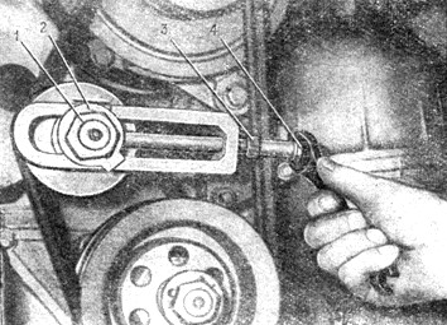
\includegraphics[width=0.7\textwidth]{src/tie.png}
            \caption{Регулировка натяжения ремней привода генератора}
            \label{tie}
        \end{center}
        \legend\centering
        1~--- гайка крепления оси натяжного ролика; 2~--- стопорная шайба; 3~--- контргайка; 4~--- регулировочный болт

    \end{figure}

    \item Отрегулировать натяжение ремня привода генератора, вращая регулировочный болт 4, пока прогиб не будет составлять требуемой величины. 
    \item Затянуть гайку 1 крепления оси натяжного ролика, загнуть края стопорной шайбы 2 и затянуть контргайку 3 регулировочного болта 4. 
    \item Поставить на место и закрепить заднюю панель ограждения двигателя. 
\end{enumerate}


\techcardsection{Проверка и регулировка натяжения ремня привода водяного насоса}

Исполнитель: механик-водитель (механик). 

Инструмент и приспособления: ключи гаечные 11 и 27~мм; линейка металлическая. 

Норма времени~--- 15 мин. 

\subsubsection{Содержание работ и технические условия}
\begin{enumerate}
    \item Снять заднюю панель ограждения двигателя. 
    \item Проверить натяжение ремня привода водяного насоса. При нормальном натяжении ремня прогиб в середине  ветви при усилии 3 кгс должен быть \range{10}{15}~мм
    \item Для натяжения ремня отвернуть гайки крепления боковины 1 (рис.~\ref{tie_2}) шкива 2 и снять \range{одну}{две} регулировочные прокладки 3. 
    
    \begin{figure}
        \begin{center}
            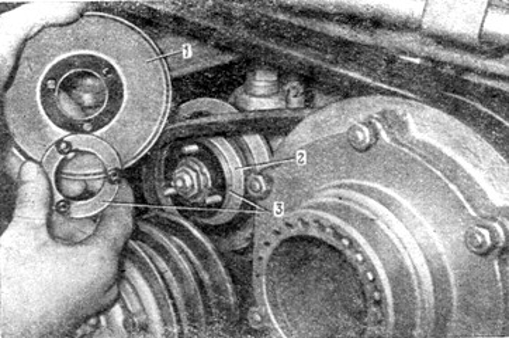
\includegraphics[width=0.7\textwidth]{src/tie_2.png}
            \caption{Регулировка натяжения ремня водяного насоса}
            \label{tie_2}
        \end{center}
        \legend\centering
        1~--- боковина; 2~--- шкив; 3~--- регулировочные прокладки
    \end{figure}

    \item \begin{enumerate}
        \item Поставить их на наружную сторону боковины и завернуть гайки, проворачивая шкив после затяжки каждой гайки. 
        \item Проверить, нормально ли натянут ремень. 
    \end{enumerate}
    \note{Регулировочные прокладки со шкива не снимать, так как при замене старого ремня новым все прокладки, нужно поставить между ступицей и съемной боковиной шкива.}
    \item Поставить и закрепить заднюю панель ограждения двигателя. 

\end{enumerate}


\techcardsection{Проверка и регулировка натяжения ремня привода компрессора}

Исполнитель: механик-водитель (механик). 

Инструмент и приспособления: ключи гаечные 17$\times$19, и 27$\times$32~мм; линейка металлическая. 

Норма времени~--- 15~мин. 

\subsubsection{Содержание работ и технические условия}
\begin{enumerate}
    \item Поднять крышку люка моторного отделения и зафиксировать ее в открытом положении стопором, снять заднюю панель ограждения двигателя. 
    \item Проверить натяжение ремня привода компрессора. Нормальный прогиб ремня на середине короткой ветви при нажатии с усилием 3 кгс должен быть \range{5}{8}~мм (рис.~\ref{tie_3}). 
    
    \begin{figure}
        \begin{center}
            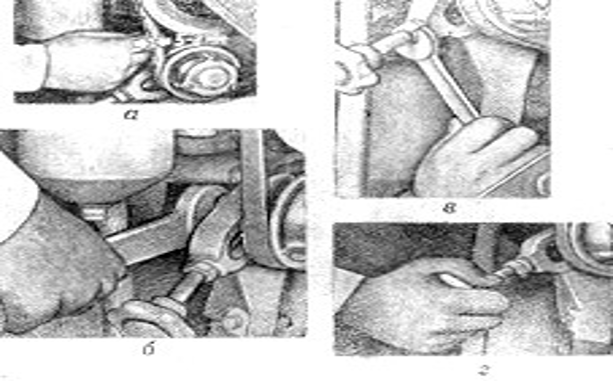
\includegraphics[width=0.75\textwidth]{src/tie_3.png}
            \caption{Регулировка натяжения ремня компрессора}
            \label{tie_3}
        \end{center}
        \legend
        \textit{а}~--- проверка натяжения ремня компрессора; \textit{б}~--- отвертывание гайки крепления оси шкива; \textit{в}~--- отвертывание гайки натяжного болта; \textit{г}~--- регулировка натяжного ремня компрессора     
    \end{figure}


    \item Для регулировки натяжения ремня ослабить гайку крепления оси шкива натяжного устройства и гайку болта-натяжителя. 
    \item Вращая болт-натяжитель по ходу часовой стрелки, отрегулировать натяжение ремня. 
    \item Затянуть гайки крепления оси шкива и болта-натяжителя. 
    \item Поставить заднюю панель ограждения двигателя, закрыть крышку люка, освободив крышку от стопора. 

\end{enumerate}


\techcardsection{Проверка и регулировка натяжения ремней привода вентилятора}
Исполнитель: механик-водитель (механик). 

Инструмент и приспособления: ключи гаечные 17$\times$19~мм; отвертка большая, линейка. 

Норма времени~--- 10 мин. 

\subsubsection{Содержание работ и технические условия}
\begin{enumerate}
    \item Снять заднюю панель ограждения двигателя.  
    \item Проверить натяжение ремней привода вентилятора. 
    При нормальном натяжении прогиб ремня в средней части верхней ветви при нажатии большого пальца руки с усилием 4 кгс должен быть в пределах \range{8}{14}~мм. 
    \item Натяжение ремня 2 (рис.~\ref{natyag}) осуществляется сжатием пружины 6 натяжного ролика 1. 
    
    \begin{figure}
        \begin{center}
            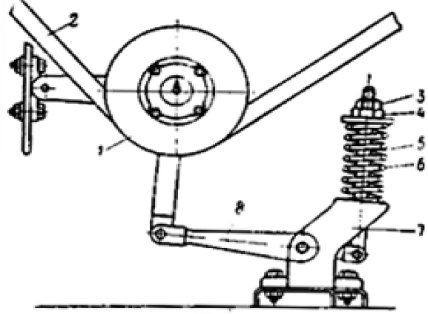
\includegraphics[width=0.8\textwidth]{src/natyag.png}
            \caption{Натяжной механизм привода вентилятора}
            \label{natyag}
        \end{center}
        \legend\centering
        1~--- натяжной ролик; 2~--- ремень; 3~--- контргайка; 4~--- гайка; 5~--- стержень; 6~--- пружина; 7~--- кронштейн; 8~--- рычаг
    \end{figure}

    \item Для регулировки натяжения ремней отвернуть на \range{три}{четыре} оборота контргайку 3 стержня 5 и гайкой 4, сжимая или отпуская пружину 6, отрегулировать натяжение ремней. 	 
    \item Завернуть контргайку 3. 
    \item Поставить на место заднюю панель ограждения двигателя. 
\end{enumerate}



\techcardsection{Регулировка клапанного механизма}
Исполнитель: механик-водитель и механик. 

Инструмент и приспособления: ключи гаечные 14, 19 и 32~мм, головка на 32~мм; вороток, отвертка, щуп, динамометр, специальный ключ для проворачивания коленчатого вала. 

Норма времени: 
\begin{itemize}
    \item для механика-водителя~---  20~мин, 
    \item для механика~--- 60~мин
\end{itemize}


\subsubsection{Содержание работ и технические условия}
\begin{enumerate}
    \item Поднять крышку люка моторного отделения и зафиксировать ее в открытом положении стопором. 
    \item Снять заднюю и боковую панели ограждения двигателя. 
    \item Отсоединить дренажную трубку от маслозаливной горловины крышки головки левого ряда цилиндров. 
    \item Выключить подачу топлива скобой регулятора. 
    \item Отвернуть барашки крепления крышек головок цилиндров и снять крышки. 
    \item Проверить момент затяжки болтов крепления осей коромысел, который должен быть \range{12}{16}~кгсм. 
    \item Проворачивая коленчатый вал по ходу часовой стрелки (если смотреть со стороны вентилятора) ключом за болт крепления шкива, установить клапан 1-го цилиндра на момент полного закрытия (момент полного поднятия), после чего провернуть коленчатый вал дополнительно на 1/3 оборота. 
    \item Проверить щупом зазор между торцом клапана и носком коромысла у впускного и выпускного клапанов первого цилиндра и при необходимости отрегулировать. 
    
    \begin{figure}
        \begin{center}
            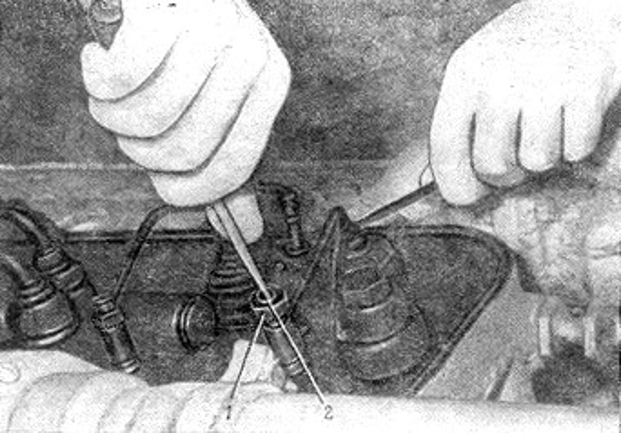
\includegraphics[width=\textwidth]{src/zazor.png}
            \caption{Регулировка зазоров клапанного механизма}
            \label{zazor}
        \end{center}
        \legend\centering
        1~--- контргайка; 2~--- регулировочный винт 
    \end{figure}
    
    \item 
    \begin{enumerate} 
        \item Для регулирования зазоров~--- ослабить контргайку 1 (рис.~\ref{zazor}) регулировочного винта 2, вставить в зазор щуп и, вращая винт отверткой, установить зазор \range{0,25}{0,3}~мм. 
        \item Придерживая винт отверткой, затянуть контргайку и проверить величину зазора. 
    \end{enumerate}


    \textit{Примечания:} 
    \begin{itemize}
        \item \textit{Щуп толщиной 0,25~мм должен входить в зазор с легким нажимом, толщиной 0,3~мм~--- с усилием.}
        \item \textit{Регулировать на холодном двигателе по истечении 30~мин после его остановки.}
    \end{itemize}
    \item В порядке работы цилиндров двигателя 1-5-4-2-6-3-7-8 проверить и при необходимости отрегулировать клапанные зазоры в соответствии с пп.~7, 8 и 9. 
    \item Пустить двигатель и прослушать его работу. При появлении стука клапанов-двигатель остановить и вновь проверить зазоры. 
    \item Поставить и закрепить крышки головок цилиндров, подсоединить и поставить снятые детали. 
    \item Поставить на место боковую и заднюю панели ограждения двигателя. 
    \item Закрыть крышку люка, освободив от стопора. 
\end{enumerate}

\techcardsection{Проверка и регулировка угла опережения впрыска топлива}
Исполнитель: механик, механик-водитель. 

Инструмент и приспособления: ключи 10, 17 и 19~мм, специальный ключ для проворачивания коленчатого вала; моментоскоп, плоскогубцы. 

Норма времени:
\begin{itemize}
    \item для механика~--- 20~мин, 
    \item для механика-водителя~--- 15~мин. 
\end{itemize} 

\subsubsection{Содержание работ и технические условия}

\begin{enumerate}
    \item Поднять крышку люка моторного отделения и зафиксировать ее в открытом положении стопора. Снять крышку люка для слива масла из картера двигателя. 
    \item Убедиться в правильном взаимном расположении меток на муфте 1 (рис.~\ref{labels}) опережения впрыска топлива и ведущей полумуфте 2 валика привода топливного насоса. Метки должны быть совмещены. 
    
    \begin{figure}
        \begin{center}
            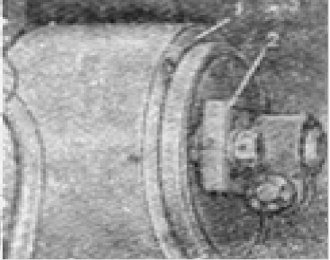
\includegraphics[width=0.65\textwidth]{src/labels.png}
            \caption{Совмещение меток}
            \label{labels}
        \end{center}
        \legend\centering
        1~--- автоматическая муфта опережения впрыска топлива; 2~--- ведущая полумуфта валика привода топливного насоса
    \end{figure}


    \item Отсоединить трубку высокого давления от штуцера (рис.~\ref{otvertyvanie}) первой секции топливного насоса. 
    
    \begin{figure}
        \centering
        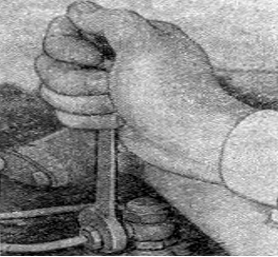
\includegraphics[width=0.65\textwidth]{src/otvertyvanie.png}
        \caption{Отвертывание гайки трубки высокого давления}
        \label{otvertyvanie}
    \end{figure}


    \item Установить моментоскоп (рис.~\ref{momentoskop}) на штуцер первой секции. 

        \begin{figure}
            \begin{center}
                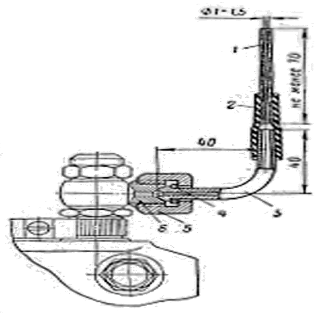
\includegraphics[width=0.7\textwidth]{src/momentoskop.png}
                \caption{Установка моментоскопа на штуцер первой секции}
                \label{momentoskop}
            \end{center}
            \legend
            1~--- стеклянная трубка; 2~--- переходная трубка; 3~--- отрезок топливопровода высокого давления; 4~--- шайба; 5~--- накидная гайка; 6~--- штуцер первой секции
        \end{figure}


    \item Включить подачу топлива скобой регулятора.
    \item Прокачать топливом систему питания двигателя ручным топливоподкачивающим насосом, предварительно ослабив одну из пробок для выпуска воздуха из корпуса топливного насоса высокого давления. Прокачивать до тех пор, пока в вытекающем топливе не исчезнут пузырьки воздуха, затем надежно затянуть пробку.
    \item Вращать коленчатый вал двигателя по ходу часовой стрелки (если смотреть со стороны вентилятора) до появления топлива в стеклянной трубке 1 моментоскопа. Вылить излишки топлива из стеклянной трубки легким встряхиванием ее.
    \item Провернуть коленчатый вал против хода примерно на 1/8 оборота. Медленно проворачивая по часовой стрелке коленчатый вал двигателя, внимательно следить за уровнем топлива в стеклянной трубке 1. В момент начала движения топлива в трубке 1 прекратить вращение вала и проверить взаимное расположение меток. 
        
    Риска на шкиве коленчатого вала должна находиться против риски с цифрой на крышке шестерен распределения или риска с цифрой на маховике должна совпадать с указателем 1 (рис.~\ref{sovmeschenie}) картера маховика. 

    Цифра у риски должна соответствовать цифре, выбитой на торце муфты (рис.~\ref{labels}). 

    \begin{figure}
        \begin{center}
            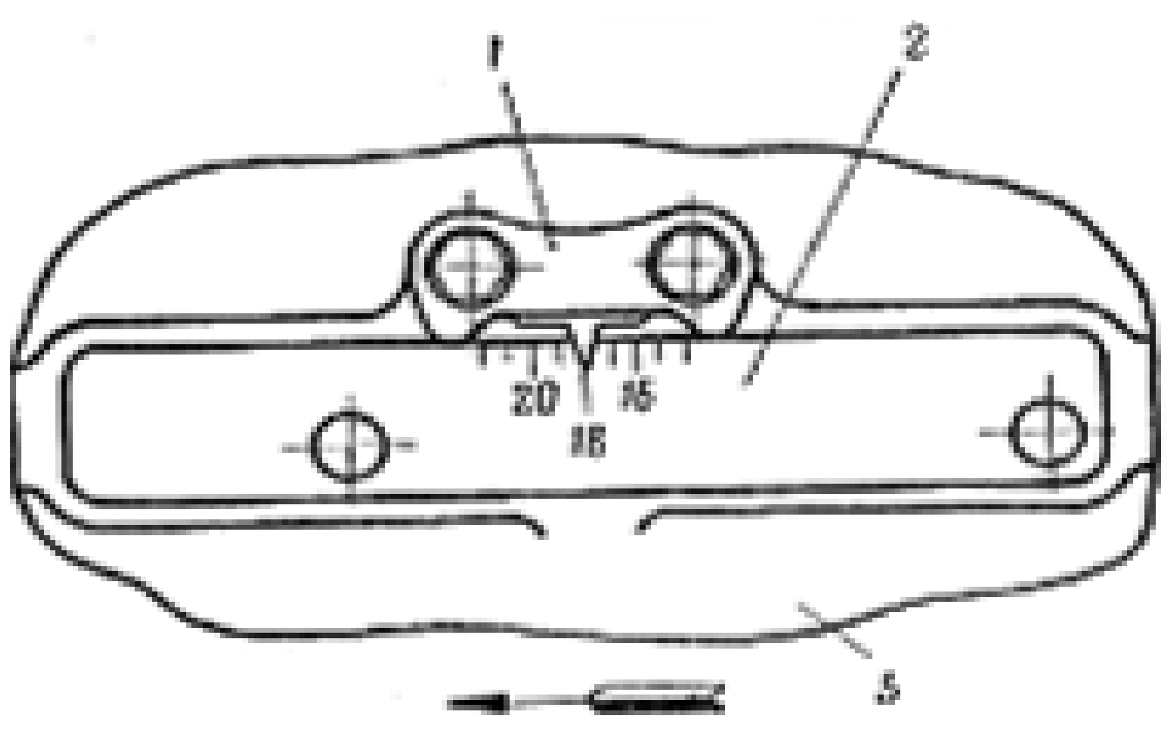
\includegraphics[width=0.8\textwidth]{src/sovmeschenie.png}
            \caption{Совмещениеие рисок на маховике с указателем картера маховика}
            \label{sovmeschenie}
        \end{center}
        \legend\centering
        1~--- указатель картера маховика; 2~--- маховик; 3~--- картер маховика
    \end{figure}

    \item Если к моменту начала движения уровня топлива в трубке указанного совмещения не произошло, необходимо расшплинтовать и ослабить болты крепления муфты валика привода топливного насоса, повернуть полумуфту валика привода на ее фланце против направления вращения, затянуть болты крепления и вновь повторить установку угла опережения впрыска топлива. При проходе рисками совмещенного положения~---- полумуфту валика привода следует повернуть на фланце по направлению ее вращения. 

    Несовпадение рисок должно быть не больше одного градуса (одно деление). 

    Смещение полумуфты относительно ее фланца на одно деление соответствует четырем делениям на маховике или крышке шестерен распределения. 
    \item После окончания регулировки угла опережения затянуть и зашплинтовать болты крепления муфты и заметить взаимное расположение рисок на муфте валика привода и на ее фланце. 
    \item Снять моментоскоп, присоединить трубку высокого давления к штуцеру первой секции топливного насоса. 
    \item Поставить заднюю панель ограждения двигателя, опустить крышку люка моторного отделения, освободив от стопора. Поставить крышку люка для слива масла из картера двигателя
\end{enumerate}



\techcardsection{Снятие и установка топливного насоса высокого давления на двигатель}
Исполнитель: механик, механик-водитель. 

Инструмент и приспособления: ключи гаечные 12, 14, 17 и 19~мм, специальный ключ для проворачивания коленчатого вала; плоскогубцы, отвертка, моментоскоп, щуп пластинчатый. 

Норма времени:
\begin{itemize}
    \item для механика~--- 30~мин, 
    \item для механика-водитля~--- 60~мин. 
\end{itemize} 

\subsubsection{Содержание работ и технические условия}
\begin{enumerate}
    \item Поднять крышку люка моторного отделения и зафиксировать в открытом положении стопором, снять заднюю панель ограждения двигателя. 
    \item Отсоединить трубку высокого давления от штуцера первой секции топливного насоса, установить моментоскоп на штуцер; проворачивая коленчатый вал, установить начало подачи топлива первой секцией топливного насоса, снять моментоскоп. 
    \item Ослабить хомуты крепления воздушного шланга к компрессору, отсоединить шланг от переходника впускных трубопроводов. 
    \item Отвернуть болты крепления переходника впускных трубопроводов, ослабить хомуты крепления патрубка переходника и воздухоочистителя, снять переходник с двигателя, закрыть впускные окна коллекторов деревянными пробками. 
    \item Отсоединить топливные трубки высокого давления от штуцеров секций топливного насоса высокого давления. 
    \item Отсоединить топливопроводы от насоса высокого давления и топливоподкачивающего насоса к фильтру тонкой очистки топлива. 
    \item Отсоединить от топливоподкачивающего насоса сливную трубку и топливопровод к фильтру грубой очистки топлива. 
    \item Отсоединить тяги от рычага управления регулятором и скобы кулисы. 
    \item Расшплинтовать и отвернуть соединительные болты ведущей полумуфты привода и муфты опережения впрыска топлива, снять болты, разъединить муфту опережения впрыска топлива с ведущей полумуфтой привода. 
    \item Отвернуть болты крепления насоса и снять насос высокого давления с двигателя (проверять и регулировать насос на специальном стенде в мастерской). 
    \item При установке нового насоса, отремонтированного или отрегулированного на стенде, обратить внимание на совмещение меток муфты опережения впрыска и ведущей полумуфты привода в момент начала подачи топлива первой секцией насоса высокого давления, а также на наличие масла в муфте опережения впрыска. 
    \item Закрепить насос высокого давления болтами в развале блока цилиндров. 
    \item Соединить муфту опережения впрыска с ведущей полумуфтой привода насоса, проверить и установить торцевой зазор в приводе топливного насоса высокого давления. Торцевой зазор регулируется осевым перемещением полумуфты по ведущему валу привода топливного насоса при отпущенной гайке болта клеммового соединения полумуфты. По окончании регулировки гайку болта клеммового соединения надежно затянуть и зашплинтовать. 
        
    Зазор между торцами кулачков ведущей полумуфты и передним концом муфты опережения, так же, как и зазор между кулачками муфты опережения и задним торцом ведущей полумуфты должен быть не менее 0,3~мм. 
        
    Проверка обязательна для всех четырех кулачков. 
    \item Подсоединить тяги к рычагу управления регулятором и скобе кулисы. 
    \item Подсоединить к топливоподкачивающему насосу сливную трубку и топливопроводы от фильтров тонкой и грубой очистки топлива. 
    \item Подсоединить топливопроводы от фильтра тонкой очистки к насосу высокого давления. 
    \item Подсоединить топливные трубки высокого давления к штуцерам секций топливного насоса за исключением первой. 
    \item Установить моментоскоп на штуцер первой секции топливного насоса высокого давления, проверить и в случае необходимости отрегулировать угол опережения впрыска топлива (см. технологическую карту №\ref{techcard13}).  
    \item Поставить и закрепить переходник на двигатель, предварительно удалив деревянные пробки из впускных окон коллекторов, соединить его с воздухоочистителем, закрепить воздушный шланг компрессора к переходнику.  
    \item Поставить заднюю панель ограждения двигателя и закрыть крышку люка моторного отделения, освободив от стопора. 
\end{enumerate}


\techcardsection{Снятие и установка форсунок на двигатель}
Исполнитель: механик-водитель. 

Инструмент и приспособлени: ключи гаечные 14, 17 и 19~мм, ключ накидной 19~мм; вилка для снятия форсунок. 

Норма времени~--- 20~мин. 

\subsubsection{Содержание работ и технические условия}
\begin{enumerate}
    \item Поднять крышку люка моторного отделения и зафиксировать в открытом положении стопором, снять боковую панель ограждения двигателя. 
\item Отвернуть барашки крепления крышки головки блока и снять ее. 
\item Отвернуть трубки отвода избыточного топлива от форсунок. 
\item Отвернуть накидную гайку топливной трубки форсунки, навернуть колпачки на штуцер форсунки и ниппель топливной трубки. 
\item \begin{enumerate}
    \item Отвернуть гайку скобы крепления форсунки (рис.~\ref{gayka_1}), снять скобу, снять форсунку (рис.~\ref{gayka_2}), закрыть деревянной пробкой гнездо форсунки. 
    \item Снятые форсунки пронумеровать в соответствии с цилиндрами двигателя с целью обеспечения установки их в те же цилиндры после обслуживания. 
\end{enumerate}

\begin{figure}
    \centering
    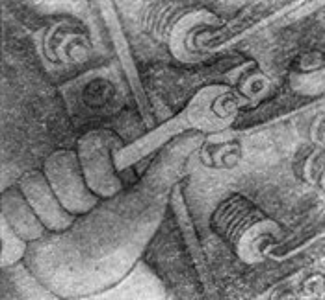
\includegraphics[width=0.65\textwidth]{src/gayka_1.png}
    \caption{Отвертывание гайки скобы форсунки}
    \label{gayka_1}
\end{figure}
\begin{figure}
    \centering
    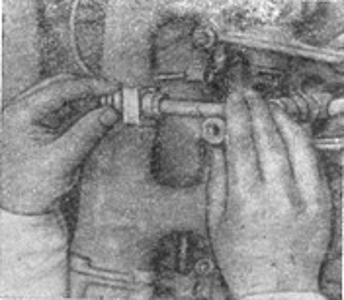
\includegraphics[width=0.65\textwidth]{src/gayka_2.png}
    \caption{Снятие форсунки}
    \label{gayka_2}
\end{figure}

\item Перед, установкой проверенной и отрегулированной или новой форсунки вынуть деревянную пробку из гнезда форсунки, тщательно протереть гнездо и коническую часть форсунки, проверить наличие медной прокладки в стакане; установить на место форсунку и скобу крепления, затянуть гайку. 
\item Снять защитные колпачки со штуцера форсунки и ниппеля топливной трубки, установить топливную трубку на место и соединить ее накидной гайкой со штуцером форсунки. 
\item Установить на место и закрепить трубки отвода избыточного топлива от форсунок. 
\item Поставить на место и закрепить болтами крышку головки блока цилиндров. 
\item Поставить на место боковую панель ограждения двигателя, опустить крышку люка моторного отделения, освободив от стопора. 

\end{enumerate}


\techcardsection{Регулировка привода управления двигателем}
\subsection{Эксплуатационная}
Исполнитель: механик-водитель. 

Инструмент и приспособление: ключ 14~мм, щуп.

Норма времени~--- 8 мин. 

\subsubsection{Содержание работ и технические условия}

\begin{enumerate}
    \item Поднять крышку надмоторного люка и закрепить ее в открытом положении стопором. 
    \item Нажать на педаль 2 (рис.~\ref{privod}) подачи топлива до упора в опорный болт 1 (максимальная подача топлива). При этом зазор между штифтом рычага 14 и болтрм 15 ограничения оборотов должен быть \range{0}{1,2}~мм. 
    
    \begin{figure}
        \begin{center}
            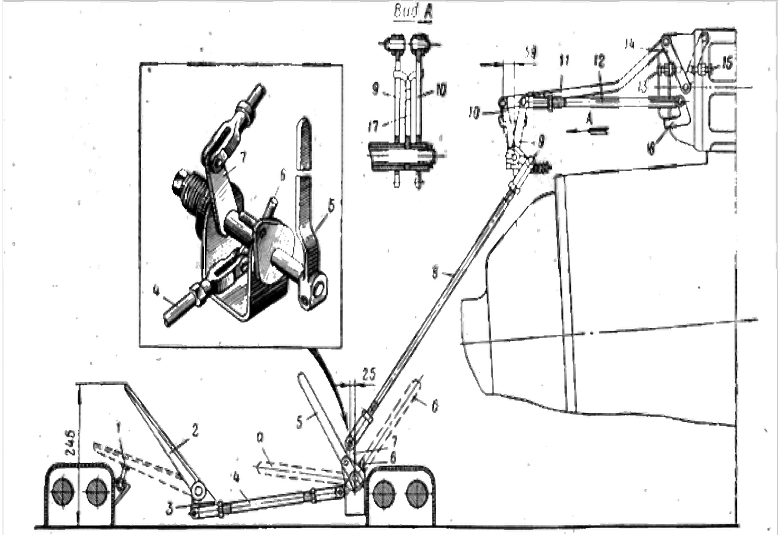
\includegraphics[width=\textwidth]{src/privod.png}
            \caption{Схема регулировки привода управления двигателем}
            \label{privod}
        \end{center}
        \legend
        1~--- болт упорный; 2~--- педаль подачи топлива; 3~--- рычаг педали; 4~--- тяга педали; 5~--- рукоятка ручной подачи топлива; 6 и 7~--- рычаги промежуточного валика; 8~--- вертикальная тяга; 9~--- рычаг управления остановки; 10~--- рычаг управления регулятором; 11~--- тяга регуля-тора; 12~--- тяга останова; 13~--- болт ограничения минимальных оборотов; 14~--- рычаг регулятора; 15~--- рычаг ограничения максимальных оборотов; 16~--- скоба установа двигателя; 17~--- промежуточный рычаг; а~--- рукоятка при максимальной подаче; б~--- рукоятка при остановке двигателя
    \end{figure}

    \item При увеличении зазора более 1,2~мм болт 1 ввинтить до обеспечения заданного зазора \range{0}{1,2}~мм. 
    \item При уменьшении зазора до 0 болт 1 вывернуть до упора его в педаль. 
    \item Закрыть надмоторный люк, освободив его от стопора.
    
\end{enumerate}
\note{На транспортере-тягаче МТ-Л порядок эксплуатационной регулировки привода двигателей аналогичен.}

\subsection{Монтажная}
Исполнители: механик и механик-водитель. 

Инструмент и приспособления: ключи гаечные. 12, 14, 17 и 19~мм; отвертка, плоскогубцы, линейка, щуп. 

Норма времени: 
\begin{itemize}
    \item для механика-водителя~--- 25~мин. 
    \item для механика~--- 15~мин
\end{itemize}

\subsubsection{Содержание работ и технические условия}
\begin{enumerate}
    \item Поднять крышку надмоторного люка и закрепить ее в открытом положении стопором. Снять переднюю панель ограждения двигателя. 
    \item Отсоединить тяги 11 регулятора и 12 останова от их рычагов 10 и 9. 
    \item Установить рычаг 10 так, чтобы ось его пальца находилась на расстоянии 39~мм от вертикальной линии, проходящей через ось вращения этого рычага. 
    \item Установить рычаг 14 регулятора в положение, соответствующее минимальной подаче (рычаг 14 регулятора должен упираться в болт 13 ограждения числа оборотов) и, отрегулировав длину тяги 11, соединить ее с рычагом 10, установив палец отверстием под шплинт влево. 
    \item Подвести рычаг 17 до упора усиком в рычаг 10. 
    \item Медленно перемещать тягу 12 вперед и в момент увеличения усилия на перемещение тяги соединить ее с рычагом 9, который должен быть подведен к другому усику рычага 17. Палец установить отверстием под шплинт вправо. 
    \item После регулировки положение рычагов должно быть: рычаг 14 штифтом упирается в болт 13; рычаг 10 упирается в один усик, а рычаг 9~--- в другой усик рычага 17; рычаги 9, 17 и 10 находятся в одной плоскости и наклонены вперед на 39~мм. 
    
    \note{На рис.~\ref{privod} рычаги 9 и 10 условно смещены относительно друг друга.}

    \item При положении рычагов 9, 10, 14 и 17 как указано в п.~7, изменением длины тяги 8 установить рычаг 7 так, чтобы ось его пальца была отклонена на 25~мм вперед от оси вращения рычага, а изменением длины тяги 4 установить педаль 2 так, чтобы конец ее был на расстоянии 246~мм от днища. 
    \item В положении максимальной подачи педаль 2 должна упираться в опорный болт 1, при этом зазор между штифтом рычага 14 и болтом 15 ограничения максимальных оборотов должен быть не более 1,2~мм. 
    \item Отрегулировав привод управления двигателем, затянуть контргайки тяг и развести шплинты на соединительных пальцах. 
    \item Закрыть крышку надмоторного люка и поставить панель ограждения двигателя. 
\end{enumerate}



\techcardsection{Регулировка привода управления коробкой передач}
Исполнители: механик и механик-водитель. 

Инструмент и приспособления: ключи гаечные 19 и 24~мм; плоскогубцы, стержень, выставки рычагов и поводков 

Норма времени: 25~мин

\subsubsection{Содержание работ и технические условия}
\begin{enumerate}
    \item Открыть люк отсека силовой передачи и зафиксировать его в поднятом положении. 
\end{enumerate}

\paragraph{Для всех передач}
\begin{enumerate}
\item Установить рычаг 2 (рис.~\ref{kpp}) переключения в нейтральное положение, совместить метки 12 на рычаге валика блокировки и корпусе колонки 1. 
\item Расшплинтовать необходимые соединительные пальцы 7. 
\item Заменить соединительный палец 7 у рычага соответствующей регулируемой передачи стержнем 11 выставки рычагов и поводков. 
\item Проверить положение заостренного конца стержня 11 выставки рычагов и поводков относительно углубления с отметкой Н (нейтральное положение) на крышке картера главной передачи. 
\item Ввинчивая или вывинчивая регулировочную вилку 5, подобрать длину регулируемой тяги 4 так, чтобы заостренный конец стержня 11 входил в углубление с отметкой Н на крышке картера главной передачи.
\end{enumerate}

    
\paragraph{Для III, IV, V и VI передач}
\begin{enumerate}
\item Проверить положение стержня 11 выставки рычагов, и поводков относительно отметок включенного положения передач на крышке картера главной передачи при включенном положении рычага 2 переключения. 
\item При несовпадении заостренного конца стержня 11 с отметками и при самовыключении передач ввинчиванием резьбовых наконечников 10 рычагов 8 и 9 добиться полного включения муфт регулируемых передач и совпадения меток с заостренным концом стержня 11. 
\item Отрегулировав привод, необходимо окончательно проверить правильность регулировки, после чего заменить стержень 11 соединительным пальцем, затянуть контргайки, а соединительные пальцы 7 зашплинтовать. Отрегулированный привод при прокрутке силовой передачи должен обеспечивать: 
    \begin{itemize}
        \item легкое, с равномерным усилием переключение передач; 
        \item свободное, без заеданий в прорезях поводков 3 и колонки 1, перемещение рычага переключения передач; 
        \item свободный проход соединительного пальца 7 в отверстия вилок и рычагов от усилия руки при нейтральном и включенном положениях рычага 2 переключения. 
    \end{itemize}
\item Закрыть люк отсека силовой передачи, предварительно освободив от стопора. 
\item Окончательно работа привода проверяется контрольным пробегом. 

\end{enumerate}

\begin{figure}
    \begin{center}
        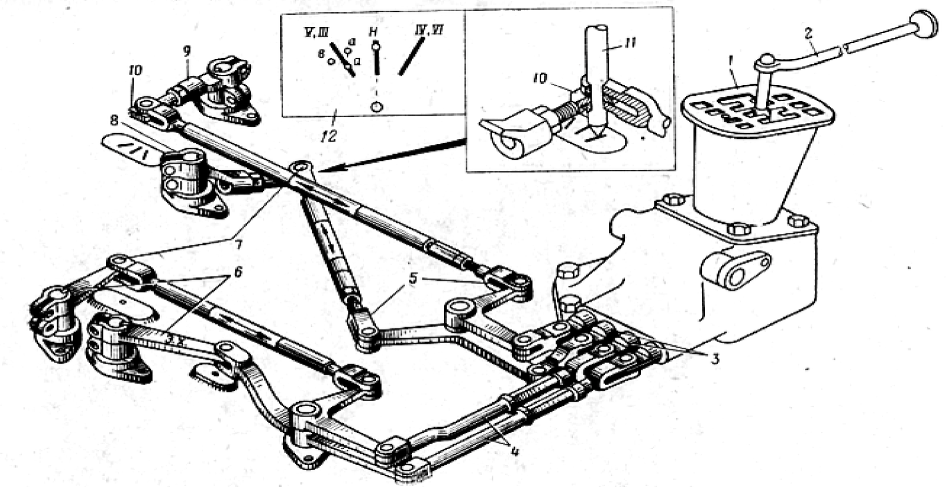
\includegraphics[width=\textwidth]{src/kpp.png}
        \caption{Схема регулировки привода управления коробкой передач}
        \label{kpp}
    \end{center}
    \legend
    1~--- колонка; 2~--- рычаг переключения; 3~--- поводки; 4~--- регулировочные тяги; 5~--- вилки регулировочные; 6~--- рычаги I--II передач и передачи заднего хода; 7~--- сосдинительные пальцы: 8~--- рычаг III--IV передач; 9~--- рычаг V--VI передач; 10~--- резьбовые наконечники рычагов: 11~--- стержень выставки рычагов и поводков; 12~--- метки на рычаге валика блокировки и корпусе колонки
\end{figure}



\techcardsection{Регулировка педали главного фрикциона и педали остановочного тормоза}

\subsubsection{Для педали главного фрикциона}
\begin{itemize}
    \item установка исходного положения; 
    \item регулировка свободного хода; 
    \item регулировка полного хода; 
    \item регулировка усилия сервопружины.
\end{itemize}

\subsubsection{Для педали остановочного тормоза}
\begin{itemize}
    \item установка исходного положения; 
    \item регулировка полного хода. 
\end{itemize}

Исполнители: механик и механик-водитель. 

Инструмент и приспособления: ключи гаечные 12, 14, 17 и 19~мм; плоскогубцы, отвертка. 

Норма времени
\begin{itemize}
    \item для механика~--- 20~мин, 
    \item для механика-водителя~--- 25~мин. 
\end{itemize}



\subsubsection{Содержание работ и технические условия}
\begin{enumerate}
    \item Снять панель двигателя над карданом. 
    \item Открыть и поставить на упор люк отсека силовой передачи. 
    \item Для установки исходного положения педали главного фрикциона необходимо: 
    \begin{enumerate}
        \item отсоединить тяги 2 (рис.~\ref{main_frick}) и 5 от двуплечего рычага вала педалей; 
        \item отрегулировать исходное положение педали главного фрикциона регулировочным болтом 4 так, чтобы расстояние от передней кромки подбашмачника педали со стороны водителя до балки было \range{72}{78}~мм; 
        \item подсоединить тяги 2 и 5 к двуплечему рычагу вала педалей, предварительно отрегулировав их; тягу 2 отрегулировать так, чтобы расстояние от горизонтальной оси качания рычага 14 блокировки кулисы до оси отверстия под палец было \range{27}{31}~мм или при наличии меток совместить метку на рычаге блокировки кулисы с меткой на корпусе колонки переключения передач; тягу 5 отрегулировать так, чтобы расстояние от вертикальной оси качания рычага 6 до оси отверстия под палец было \range{18}{22}~мм в сторону кормы транспортера-тягача. В выполнении этой операции заключается регулировка блокировки коробки передач. 
    \end{enumerate}
    \item Свободный ход педали регулируется изменением длины тяги 13 так, чтобы ее перемещение было в пределах \range{6,5}{8}~мм. 
    \item Полный ход педали регулируется регулировочным болтом 3 так, чтобы при выжиме педали до упора в болт перемещение тяги 13 составляло \range{36}{39}~мм. 
    \item Под действием сервопружины 11 педаль после снятия ноги должна самостоятельно возвращаться в исходное положение. Для этого регулируют положение кронштейна 15 сервопружины и усилие сервопружины 11. Предварительное положение кронштейна 15 сервопружины от регулировать так, чтобы при выборе свободного хода педали длинное плечо двуплечего рычага 7 и стержень 16 сервопружины составляли одну прямую. 
    Если после этого педаль будет зависать в положении выбранного свободного хода, то необходимо кронштейн 15 сервопружины сместить от его первоначального положения к корме транспортера-тягача до исключения зависания педали. 
    Усилие сервопружины и регулировать следующим образом: 
    \begin{enumerate}
        \item выжать педаль главного фрикциона до упора в регулировочный болт 3 и сжать сервопружину 11 с помощью гайки 9 так, чтобы педаль удерживалась пружиной в этом положении; 
        \item отпустить на несколько оборотов гайки сервопружины, чтобы педаль плавно возвращалась в исходное положение. 
    \end{enumerate}
    \item Исходное положение педали остановочного тормоза устанавливается после отсоединения тяги 1 аналогичного установке исходного положения педали главного фрикциона. Взаимное смещение поверхностей подбашмачников допускается не более 4~мм.  
    \item Полный ход педали остановочного тормоза определяется регулировочным болтом 3 так, чтобы при выжиме педали до упора в болт перемещение тяги 1 тормозного крана было \range{35}{43}~мм. После снятия ноги педаль должна возвращаться в исходное положение.  
    \item Закрыть люк отсека силовой передачи, освободив от стопора, поставить на место панель двигателя над карданом. 
\end{enumerate}

\begin{figure}
    % TODO: повернуть картинку, чтобы сделать покрупнее
    \begin{center}
        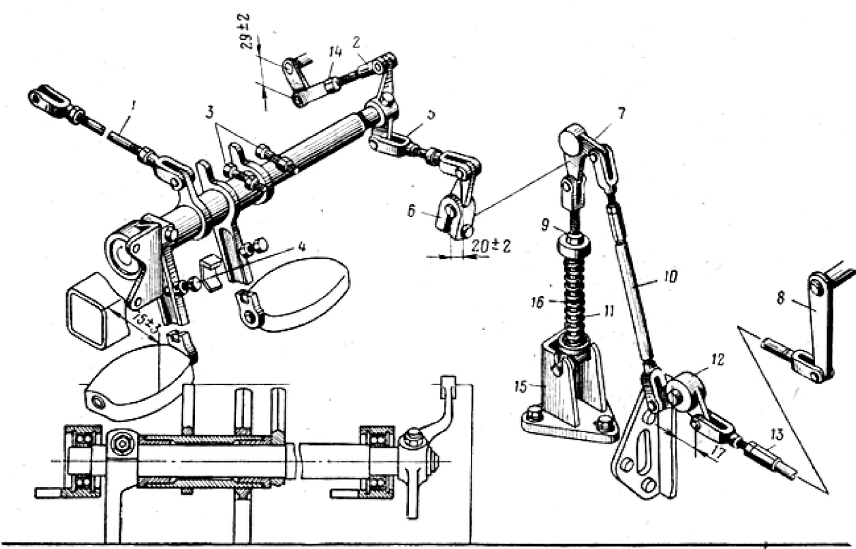
\includegraphics[width=\textwidth]{src/main_frick.png}
        \caption{Схема регулировки педали главного фрикциона и педали остановочного тормоза}
        \label{main_frick}
    \end{center}
    \legend
    1~--- тяга тормозного крана; 2~--- тяга блокировки; 3 и 4~--- болты регулировочные; 5~--- тяга педали; 6~--- рычаг переходной; 7 и 12~--- рычаги двуплечие; 8~--- рычат педали; 9~--- тайка регулировочная; 10~--- тяга главного фрикциона короткая; 11~--- сервоп-ружина; 13~--- тяга главного фрикциона; 14~--- рычаг блокировки; 15~--- кронштейн сервопружины; 16~--- стержень сервопружины
\end{figure}


\techcardsection{Регулировка остановочных тормозов}
Исполнитель: механик-водитель. 

Инструмент и приспособления: ключи гаечные 14 и 17~мм; щуп. 

Норма времени~--- 16~мин. 

\subsubsection{Содержание работ и технические условия}
\begin{enumerate}
    \item Открыть крышку люка отсека силовой передачи. 
    \item Отпустить контргайки регулировочных болтов 3 (рис.~\ref{tormoz}) остановочного тормоза. 
    \item Удерживая рычаг 1 тормоза в крайнем нижнем положении, при помощи регулировочной гайки 2, установить зазор между тормозным барабаном и колодками тормозной ленты \range{1,5}{2,5}~мм. Равномерный зазор устанавливается регулировочными болтами 3. Допускается местный зазор не менее 0,5~мм в \range{двух}{трех} местах. 
    \item Затянуть контргайки регулировочных болтов 3 остановочного тормоза до плотного упора.  
    \item Закрыть крышку люка отсека силовой передачи. 

\end{enumerate}

\begin{figure}
    \begin{center}
        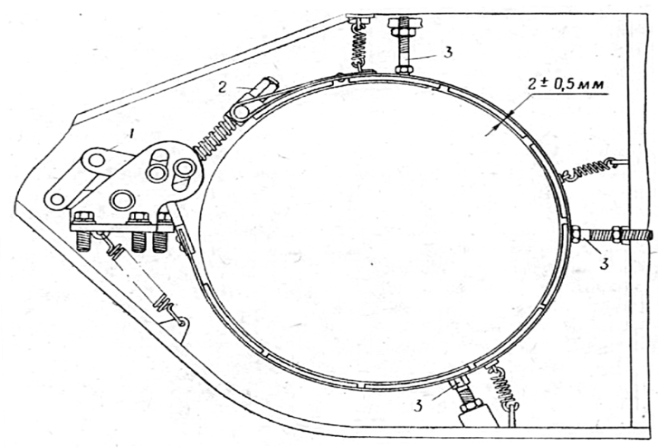
\includegraphics[width=\textwidth]{src/tormoz.png}
        \caption{Схема регулировки остановочных тормозов}
        \label{tormoz}
    \end{center}
    \legend\centering
    1~--- рычаг тормоза; 2~--- гайка регулировочная; 3~--- болты регулировочные
\end{figure}



\techcardsection{Регулировка (эксплуатационная) рычагов управления}

Исполнитель: механик-водитель. 

Инструмент и приспособления: ключи гаечные 14, 17 и 19~мм; плоскогубцы, линейка. 

Норма времени~--- 30~мин. 

\subsubsection{Содержание работ и технические условия}
\begin{enumerate}
    \item Отсоединить тягу 1 (рис.~\ref{rychag}) от промежуточного рычага. 
    \item Установить регулировочные болты 2 так, чтобы при упоре в них выступов рычагов 3 управления рукоятки рычагов отстояли от балки на 90- 100~мм. При этом взаимное смещение положения рукояток рычагов 3 управления допускается не более 3~мм. 
    \item Отрегулировать длину тяги 1 и соединить ее с промежуточным рычагом. При этом ролики рычагов тормозов механизма поворота должны находиться в соответствующих лунках на профильной поверхности кулаков, как указано на рис.~\ref{rychag}. 
\end{enumerate}


\begin{figure}
    \begin{center}
        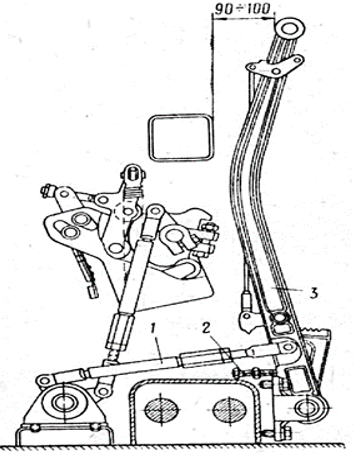
\includegraphics[width=0.6\textwidth]{src/rychag.png}
        \caption{Схема регулировки рычагов управления}
        \label{rychag}
    \end{center}
    \legend\centering
    1~--- переходная тяга; 2~--- регулировочный болт; 3~--- рычаг управления
\end{figure}


\techcardsection{Регулировка (эксплуатационная) свободного хода хвостовика поводковой коробки фрикциона механизма поворота}

Исполнитель: механик. 

Инструмент и приспособления: ключи гаечные 17 и 19~мм; плоскогубцы, линейка. 

Норма времени~--- 15~мин. 


\subsubsection{Содержание работ и технические условия}
\begin{enumerate}
    \item Открыть люк отсека силовой передачи. 
    \item Установить рычаги управления в переднее крайнее положение; при этом ролики рычагов тормозов механизмов поворота должны находиться в соответствующих лунках на профильной поверхности кулаков. 
    \item Проверить свободный ход поводковой коробки, для чего: шарнирную тягу 3 (рис.~\ref{frick_box}) фрикциона механизма поворота с хвостовиком поводковой коробки 1 подать до отказа назад, а затем вперед и по перемещению соединительного пальца 2 замерить величину свободного хода. Свободный ход должен быть в пределах \range{7}{9}~мм. 
    \item Если свободный ход поводковой коробки 1 больше или меньше указанных величин, то отрегулировать в такой последовательности: 
    \begin{enumerate}
        \item отпустить контргайки шарнирной тяги 3 и, вращая тягу, добиться указанного свободного хода (\range{7}{9}~мм);  
        \item проверить правильность регулировки, как указано в п.~3; 
        \item затянуть контргайки шарнирной тяги 3. 
    \end{enumerate}
    \item Закрыть люк отсека силовой передачи. 
\end{enumerate}

\begin{figure}
    \begin{center}
        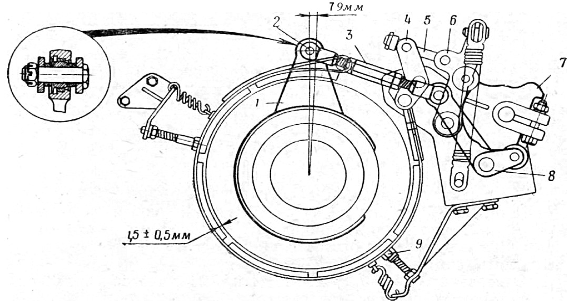
\includegraphics[width=0.9\textwidth]{src/frick_box.png}
        \caption{Схема регулировки свободного хода поводковой коробки фрикциона механизма поворота}
        \label{frick_box}
    \end{center}
    \legend 
    1~--- поводковая коробка; 2~--- соединительный палец; 3~--- шарнирная тяга; 4 и 6~--- рычаги тормоза; 5~--- регулировочная тяга; 7~--- кулак; 8~--- рычаг фрикциона; 9~--- регулировочный болт
\end{figure}


\techcardsection{Регулировка (монтажная) фрикционов механизма поворота}
Исполнитель: механик. 

Инструмент и приспособления: ключи гаечные 12, 17, 19 и 46~мм; плоскогубцы отвертка, линейка. 

Норма времени~--- 50~мин. 

\subsubsection{Содержание работ и технические условия}
\begin{enumerate}
    \item Открыть люк отсека силовой передачи. 
    \item Отогнуть замковую шайбу 7 (рис.~\ref{frick}), отвернуть гайку 8 и снять ведущий барабан 6. 
    \item Отогнуть лапки замковых шайб 10 и отвернуть шесть гаек 9 на пальцах 2 отжимного диска 3.  
    \item Снять нажимной диск 1.  
    \item Снять с каждого пальца 2 несколько регулировочных прокладок 11, 12 и 13 (суммарная толщина снятых с каждого пальца прокладок должна быть одинаковой). 
    \item Надеть нажимной диск 1 на пальцы 2 и закрепить его. 
    \item Проверить величину свободного хода поводковой коробки 5. Он должен быть \range{14}{18}~мм, после чего затянуть гайки 9 и зашплинтовать их шайбами. 
    \item Надеть ведущий барабан 6 на хвостовик вала 4 фрикциона главной передачи, закрепить его гайкой 8 и отогнуть шайбу 7. 
    \item Присоединить тягу поводковой коробки 5 к хвостовику поводковой коробки, проверить свободный ход поводковой коробки, при необходимости отрегулировать (см. технологическую карту №\ref{techcard21}). 
    \item Закрыть люк отсека силовой передачи. 
\end{enumerate}


\begin{figure}
    \begin{center}
        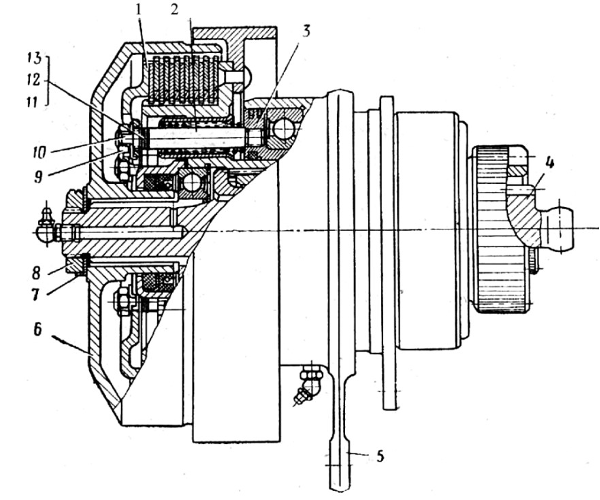
\includegraphics[width=0.9\textwidth]{src/frick.png}
        \caption{Регулировка фрикционов механизма поворота}
        \label{frick}
    \end{center}
    \legend
    1~--- нажимной диск; 2~--- палец; 3~--- отжимной диск; 4~--- вал фрикциона; 5~--- поводковая коробка; 6~--- ведущий барабан; 7 и 10~--- шайбы; 8 и 9~--- гайки; 11, 12 и 13~--- регулировочные прокладки
\end{figure}


\techcardsection{Регулировка зазора между роликом рычага тормоза механизма поворота и впадиной кулака}
Исполнитель: механик-водитель. 

Инструмент и приспособления: ключи гаечные 14 и 17~мм, щуп. 

Норма времени~--- 12~мин. 

\subsubsection{Содержание работ и технические условия}
\begin{enumerate}
    \item Открыть люк отсека силовой передачи. 
    \item Поставить рычаги управления в первое положение. 
    \item Проверить щупом наличие зазора а между роликом рычага 4 (рис.~\ref{zazor_1}) тормрза механизма поворота и впадиной кулака. Зазор а должен быть \range{2}{3}~мм. 
    \item Регулировать зазор а изменением зазора между тормозным барабаном и колодками лент тормоза механизма поворота: 
    \begin{enumerate}
        \item если зазор а мал, регулировочную гайку 2 навинтить на \range{один}{два} оборота на серьгу 1 ленты тормоза механизма поворота; 
        \item если зазор а велик, регулировочную гайку 2 свинтить на \range{один}{два} оборота с серьги 1 ленты тормоза механизма поворота. 
    \end{enumerate}
    \item Закрыть люк отсека силовой передачи. 
\end{enumerate}

\begin{figure}
    \begin{center}
        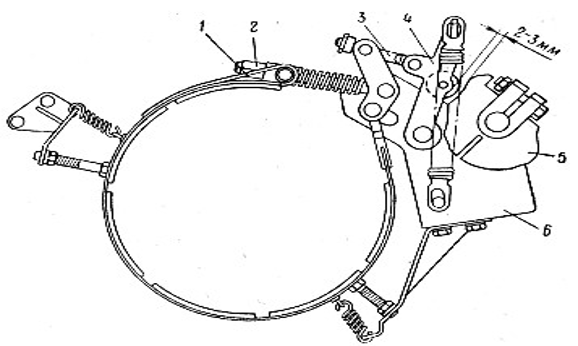
\includegraphics[width=0.9\textwidth]{src/zazor_1.png}
        \caption{Схема регулировки зазора между роликом рычага тормоза механизма поворота левого и впадиной кулака}
        \label{zazor_1}
    \end{center}
    \legend
    1~--- серьга ленты тормоза; 2~--- палец; 3~--- отжимной диск; 4~--- вал фрикциона; 5~--- поводковая коробка; 6~--- ведущий барабан; 7 и 10~--- шайбы; 8 и 9~--- гайки; 11, 12 и 13~--- регулировочные прокладки

    \note{В результате регулировки зазора между роликом рычага тормоза механизма поворота и впадиной кулака~--- зазор между тормозными барабанами механизма поворота и колодками лент устанавливается автоматически.} 
\end{figure}



\techcardsection{Регулировка приводов остановочных тормозов}
Исполнитель: механик. 

Инструмент и приспособления: ключи гаечные 12 и 14~мм; плоскогубцы. 

Норма времени~--- 20~мин.  

\subsubsection{Содержание работ и технические условия}
\begin{enumerate}
    \item Открыть люк отсека силовой передачи. 
    \item Отрегулировать положение вилки 4 (рис.~\ref{privod_setup}), свинчивая ее или навинчивая на шток тормозной камеры, так, чтобы палец 5 упирался в верхний торец прорези вилки. При этом рычаг 1 остановочного тормоза должен находиться в горизонтальном положении. 
    \item Поставить рычаги управления в первое положение. При этом рычаг 6 должен касаться своим верхним скосом соответствующего скоса рычага 7 по всей плоскости. Палец 3 рычага должен упираться в переднюю прорезь вилки 2. 
    \item Закрыть люк отсека силовой передачи Правильность регулировок приводов управления транспортером-тягачом проверяется контрольным пробегом. 
\end{enumerate}


\begin{figure}
    \begin{center}
        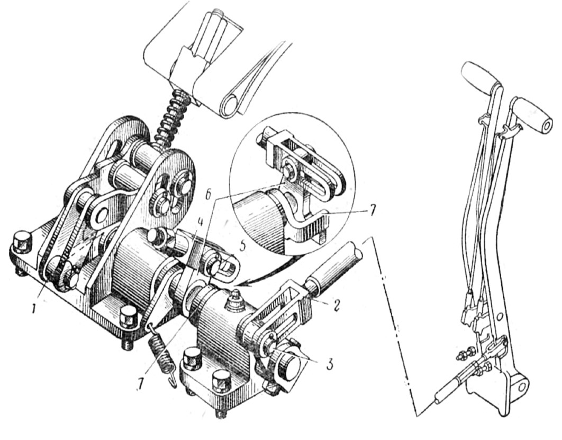
\includegraphics[width=0.9\textwidth]{src/privod_setup.png}
        \caption{Схема регулировки привода остановочных тормозов}
        \label{privod_setup}
    \end{center}
    \legend
    1~--- рычаг остановочного тормоза; 2~--- вилка тяги рычага управления; 3 и 5~--- пальцы; 4~--- вилка тяги тормозной камеры; 6 и 7~--- рычаги со скосами 

\end{figure}


\techcardsection{Регулировка натяжения гусеницы, замена трака и надевание гусеницы}
\label{process25}
Исполнитель: механик-водитель, слесарь. 

Инструмент и приспособления: ключ гаечный 19~мм; ключ специальный; выколотки пальцев короткая и длинная, кувалда, молоток, наставка специальная для расклепки пальцев. 

Норма времени:
\begin{enumerate}
    \item для механика-водителя~--- 25~мин,
    \item  для слесаря~--- 15~мин. 
\end{enumerate}



\subsubsection{Содержание работ и технические условия}

\begin{enumerate}
    \item Поставить транспортер-тягач на ровную площадку. 
    \item Затормозить одну из гусениц, поставив рычаг управления во второе положение. 
    \item
    \begin{enumerate}
        \item Выключить главный фрикцион, пустить двигатель, включить передачу заднего хода и на малых оборотах плавным включением главного фрикциона выбрать провисание гусеницы на участке между первым опорным катком и ведущим колесом незаторможенной стороны гусеницы. 
        \item\label{item_check_tension}  По расположению верхней ветви гусеницы определить правильность ее натяжения (верхняя ветвь должна лежать на четырех опорных катках, не касаясь первого и шестого катков). 
    \end{enumerate}
    \item\label{item_track_tension} Если гусеница натянута недостаточно, следует открыть люк на кормовом листе, снять стопор 1 (рис.~\ref{natyag_setup}) натяжного винта 2 и ключом вращать винт 2 по ходу часовой стрелки до нормального натяжения гусеницы. Для ослабления натяжения вращать винт 2 в противоположную сторону. 
    \item Если винт натяжного устройства завинчен до отказа, а гусеница не натянута, необходимо удалить один трак. 
    

    \begin{figure}
        \begin{center}
            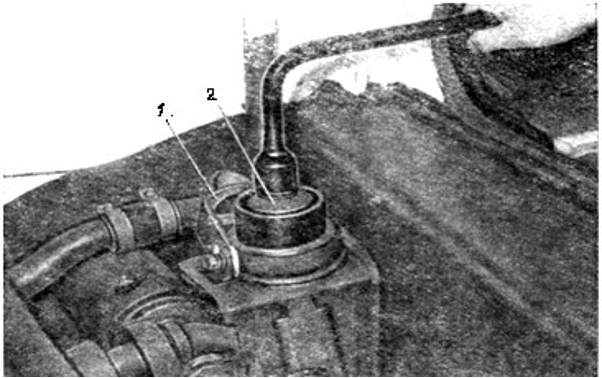
\includegraphics[width=0.9\textwidth]{src/natyag_setup.png}
            \caption{Регулировка натяжения гусеницы}
            \label{natyag_setup}
        \end{center}
        \legend\centering
        1~--- стопор; 2~--- натяжной винт

    \end{figure}


        \note{За период эксплуатации допускается удалять не более 10 траков. Гусеницы, имеющие 98 траков в каждой, подлежат замене. Удаляемые из гусеницы траки используются как запасные для замены дефектных.}
        
        Заменять дефектные траки новыми, не бывшими в эксплуатации, не рекомендуется, так как вследствие разности шага новых и бывших в эксплуатации траков возможно нарушение зацепления. 
        
        Заменять трак следует на участке между ведущим колесом и первым опорным катком в нижней ветви в следующем порядке: 
        \begin{enumerate}
            \item ослабить натяжение гусеницы (см. п.~\ref{item_track_tension}); 
            \item перемещением транспортера-тягача вывести трак, подлежащий удалению, на наклонную нижнюю ветвь между ведущим колесом и первым опорным катком; 
            \item затормозить вторую гусеницу; 
            \item на первой передаче кратковременным включением главного фрикциона натянуть верхнюю ветвь гусеницы с траком, подлежащим удалению (замене), и заглушить двигатель; 
            \item выбить пальцы и удалить (заменить) трак, после чего расклепать пальцы; 
            \item проверить натяжение гусеницы, при необходимости отрегулировать  (см. пп.~\ref{item_check_tension} и \ref{item_track_tension}). 
        \end{enumerate}


    \item При разрыве (замене) гусеница надевается в такой последовательности (при этом вторая гусеница должна быть надета): 


        \begin{enumerate}
            \item разостлать гусеницу так, чтобы траки были направлены шестью проушинами вперед (по ходу транспортера-тягача); 
            \item своим ходом (с помощью второй гусеницы) наехать на разостланную гусеницу так, чтобы впереди переднего катка оставалось два-три трака;» 
            \item пользуясь натяжным устройством, поставить направляющее колесо в крайнее переднее положение; 
            \item надеть верхнюю ветвь гусеницы на направляющее колесо, опорные катки и ведущее колесо (при надевании верхней ветви гусеницы на ведущее колесо или при снятии ее с ведущего колеса необходимо поддерживать крайний трак гусеницы, чтобы не повредить кожух гидроамортизатора); 
            \item выключить главный фрикцион, пустить двигатель, включить первую передачу, затормозить соединенную гусеницу, поставив рычаг управления во второе положение; 
            \item плавным включением главного фрикциона на малых оборотах натянуть верхнюю ветвь несоединенной гусеницы и в таком положении затормозить ее; 
            \item соединить пальцем концы гусеницы так, чтобы головка пальца находилась с наружной стороны гусеницы; 
            \item проверить правильность и при необходимости отрегулировать натяжение гусеницы, как указано в п.~4.  
        \end{enumerate}
\end{enumerate}
